\documentclass[14pt]{beamer}

\title[WTEF 2020]{Tic Tac Toe}
\subtitle{using Reinforcement Learning}
\author[Group 12]{Sanjana Chakravarty, Mahjabeen Azad, Shobhitaa Barik}
\date{August 2020}

\usetheme{Madrid}
\usecolortheme{crane}
\usepackage{textcomp}
\usepackage{xcolor}

\definecolor{myPink}{cmyk}{0, 0.7808, 0.4429, 0.1412}
\definecolor{myAmber}{rgb}{1.0, 0.49, 0.0}

\begin{document}

\begin{frame}
    \titlepage
\end{frame}

\begin{frame}{Overview}
    \begin{center}
        \textcolor{myAmber}{Player vs Computer Tic Tac Toe Game}
    \end{center}
   
    \begin{center}
    Training a tic tac toe game with reinforcement learning to improve the AI\textquotesingle s success rate with experience.
    \end{center}
\end{frame}

\begin{frame}{Reinforcement Learning}
    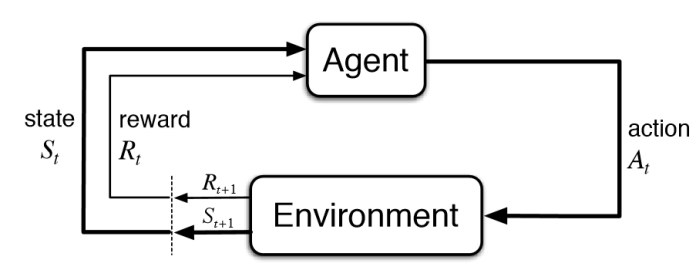
\includegraphics[width=110mm]{RL.jpg}
\end{frame}

\begin{frame}{Technology Stack/Framework}
        \begin{itemize}
            \item Language: Python
            \item Pygame for graphical interface 
            \item Pygame-menu to allow user to choose player
            \item CSV file handling
        \end{itemize}
\end{frame}

\begin{frame}{Brief Description}
        \begin{itemize}
            \item Q Learning is the algorithm used
            \item Past actions and rewards are considered
            \item Quality of every possible action from a given state is estimated
            \item Action taken by exploring and exploiting
        \end{itemize}
\end{frame}

\begin{frame}{Status}
    \begin{description}[STATUS]
        \item[\color{myPink}{24 Jun 2020}] Coded a two-player Tic Tac Toe game
        \item[\color{myPink}{27 Jun 2020}] Modified to player vs computer game
        \item[\color{myPink}{29 Jun 2020}] Read about different RL algorithms
        \item[\color{myPink}{04 Jul 2020}] Looked into different libraries
        \item[\color{myPink}{11 Jul 2020}] Implemented Q learning and interactive play
        \item[\color{myPink}{12 Jul 2020}] Used CSV file for state values
        \item[\color{myPink}{10 Aug 2020}] Implemented menu to choose player
    \end{description}
\end{frame}

\begin{frame}{Difficulties Faced}
    \begin{itemize}
        \item Maths involved in algorithms is complex
        \item Some of the algorithms are interlinked
        \item Integration of training agent with interactive play
        \item Letting player choose to play first or second
        \item Bug in training code
    \end{itemize}
\end{frame}

\begin{frame}{Learning}
    \begin{itemize}
        \item Basic machine learning algorithms
        \item Learnt how to use git
        \item Handling CSV files
        \item Using pygame module
        \item Temporal Difference learning algorithm
    \end{itemize}
\end{frame}

\begin{frame}{References}
    \begin{itemize}
        \item Reinforcement Learning: An Introduction by Barto and Sutton
        \item https://www.kaggle.com/slobo777/tic-tac-toe-agent-using-q-learning
    \end{itemize}
\end{frame}

\begin{frame}{Sneak peak into our ambitious side}
    \begin{center}
        Future Venture: \textcolor{gray}{Goats} and \textcolor{myAmber}{Tigers}
    \end{center}
\end{frame}

\end{document}
